% !TEX root =  ../main_iclr.tex



In this section we define a probabilistic model that describes the movement of electrons that define linear topology reactions.
We represent a set of molecules as a set of graphs $\moleculeSet$, with atoms $\Ac$ as vertices and bonds $\Bc$ as edges;
each connected component of the graph defines an individual molecule.
We can associate an ordering over all the atoms in all the molecules in the set using an {\em atom map} number:
an integer label assigned to each non-hydrogen atom in both the reactants and the products which 
both permits easy matching between atoms before and after the reaction, and
gives us a consistent way to index particular atoms. Molecules input into the model are first put in a Kekul\'e form, a process which makes explicit the location of single and double bonds in aromatic structures;
each bond $b \in \Bc$ is either a single, double, or triple bond.

Each atom $v \in \Ac$ includes a set of features, such as its atom type (e.g. carbon, oxygen, \dots); the full list of input atom features can be found in Table 3 of the appendix.
 However, when learning functions that operate over these atoms we do not work with these raw features directly but instead with the atom, or equivalently, node embedding. 
 These contain information about the atom of interest as well as its surrounding interest.
 These can be computed using any model that is able to compute graph-isomorphic features, for instance usually via message-passing techniques \citep{gilmer2017neural}; we choose to use 4 layer gated graph neural network (GGNN) message functions \citep{li2016gated}, for which we include a short review of in the appendix. 
 These produce a $d$-dimensional embedding of an atom and if we stack these vectors up as rows (using the atom mapping to define an order)  we have the matrix $\nodeEmbeddings{\moleculeSet_t} \subseteq \mathbb{R}^{|\Ac|\times d}$, containing all the node embeddings for a particular molecule set, $\moleculeSet_t$.





Given an initial set of reactant molecules $\moleculeSet_0$ and a set of reagent molecules $\moleculeSet_r$, 
our model defines a conditional distribution over a sequence of atoms (which we also refer to as actions) $\electronPath_{0:T} = (a_0, a_1, \ldots, a_T)$,
which fully characterizes the electron path.
This electron path in turn deterministically defines both a final product $\moleculeSet_{T+1}$, 
denoting the outcome of the reaction,
as well as a sequence of intermediate products $\moleculeSet_t$, for $t = 1,\dots,T$,
which correspond to the state of the graph after the first $t$ steps in the subsequence $\electronPath_{0:t} = (a_0, \dots, a_t)$ are applied to the initial $\moleculeSet_0$. We also define a stopping sequence $\mathcal{S}_t = (s_0, \ldots, s_{T+1})$ which indicates if the reaction should stop (i.e, $s_t\!=\!1$ if the reaction should stop and is $0$ otherwise). 

We propose to learn a distribution $p_\theta( \electronPath_{0:T} \mid \moleculeSet_0, \moleculeSet_r)$ over electron movements. 
We first detail the generative process %(i.e., the forward pass) 
that specifies $p_\theta$, before describing how to train the model's parameters, $\theta$.


\subsection{Generative process}


\begin{figure*}
\centering
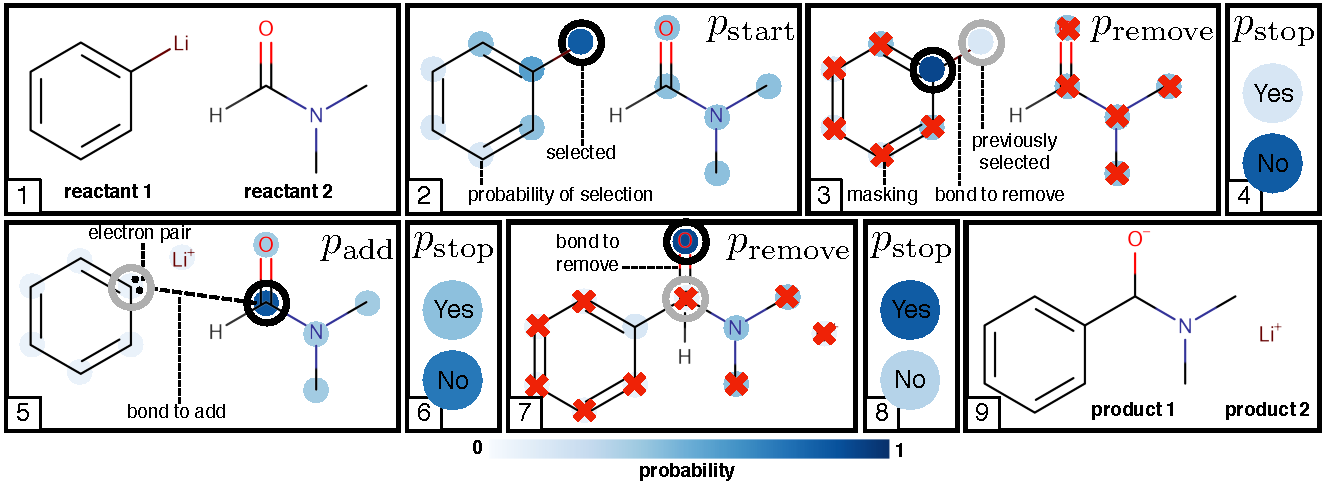
\includegraphics[width=\textwidth]{reaction_model_blue}
\caption{
 This figure shows the sequence of actions in transforming the reactants in box 1 to the products in box 9.
 The sequence of actions will result in a sequence of pairs of atoms, between which bonds will alternately be removed and created, creating a series of intermediate products. 
At each step the model sees the current intermediate product graph (shown in the boxes) as well as the previous action, if applicable, shown by the grey circle. It uses this to decide on the next action.
We represent the characteristic probabilities the model may have over these next actions as colored circles over each atom.
Some actions are disallowed on certain steps, for instance you cannot remove a bond that does not exist; these blocked actions are shown as red crosses.
}
\label{fig:reaction_model}
\end{figure*}







First note that since our reactions are a single path of electrons through the reactants then, at any point, the next step in the path depends only on (i) the intermediate molecule formed by the action path up to that point, (ii) the previous action taken (indicating where the free pair of electrons are) and (iii) the point of time through the path, indicating whether we are on an add or remove bond step. 
We make the simplifying assumption that the stop probability and the actions after the initial action $a_0$ do not depend on the reagents. This leads to a parameterized model with dependency structure:
\begin{align}
\label{eq:jointprob}
p_\theta(\electronPath_{0:T} \mid \moleculeSet_0, \moleculeSet_r) 
&=
	p_\theta(s'_0 \mid \moleculeSet_0)
	p_\theta(a_0 \mid \moleculeSet_0, \moleculeSet_r)\\ \nonumber &\quad \times
	\left[\prod_{t=1}^{T}
		p_\theta(s_{t}' \mid \moleculeSet_{t})
		p_\theta(a_t \mid \moleculeSet_{t}, a_{t-1}, t)
	\right]
	p_\theta(s_{T+1} \mid \moleculeSet_{T+1})
	,
\end{align}
where we have defined $p_\theta(s'_t \mid \moleculeSet_t) \equiv 1 - p_\theta(s_t \mid \moleculeSet_t)$ to be the probability of {\em continuing} a reaction given the current molecule set $\moleculeSet_t$.
The other terms include $p_\theta(a_0 \mid \initialAndReactants)$, the probability of the initial state $a_0$ given the reactants and reagents; 
the conditional probability $p_\theta(a_t \mid  \moleculeSet_t, a_{t-1}, t)$ 
%\todo[]{maybe somehow refer to "bond type" instead of $t$?} 
of next state $a_t$ given the intermediate products $\moleculeSet_t$ for $t > 0$;
and the probability $p_\theta(s_t \mid \moleculeSet_t)$ that the reaction terminates with final product $\moleculeSet_{t}$.


\begin{algorithm}[t]
  \caption{The generative steps of ELECTRO.}
  {\bf Input:}~~Reactant molecules $\Mc_0$ (consisting of atoms $\Ac$), reagents $\Mc_r$, atom embedding function $\fEmbed(\cdot)$, graph embedding function $r(\cdot)$, time steps $T^\mathrm{max}$
  
  \begin{algorithmic}[1]
  	\STATE $\nodeEmbeddings{\moleculeSet_0} = \fEmbed(\Mc_0)$ \COMMENT{atom embedding of reactants}
  	\STATE $\contextVect_\mathrm{reagent} = r(\Mc_r)$ \COMMENT{graph embedding of reagents}
  	%\STATE $\actionLogits = $
  	\STATE $p_{\mathrm{start}}(a_t \mid \moleculeSet_0, \moleculeSet_r) = \mbox{softmax}(\fInitial(\nodeEmbeddings{\moleculeSet_0}, \contextVect_\mathrm{reagent}))$ \COMMENT{probability $a_t$ starts the reaction}
  	\STATE $a_{0} \sim p_{\mathrm{start}}(a_t \mid \moleculeSet_0, \moleculeSet_r)$
  	\FOR{$t = 1, \ldots, T^\mathrm{max}$}
  		\STATE $\moleculeSet_t \leftarrow \moleculeSet_{0}, a_0, \ldots, a_{t-1}$ \COMMENT{modify molecules based on starting molecules and electron actions}
  		%\STATE \mathbf{h}_
  	\ENDFOR
 %  	% Set up pool of completed paths to sort later
 %  	\STATE $\outputPool = \{\left( \emptyset, \log (1 - \cProbCont(\Mc_0)) \right) \}$  \COMMENT{This set will store all completed paths.}
 %  	\STATE $\removeFlag \!=\!1$ \COMMENT{Remove flag}
  	
 %  	% Pick the first action.\\
 %  	\STATE
	% \STATE $\hat{\Bc} = \emptyset$.  \COMMENT{This set will store all possible open paths. Cleared at start of each timestep.}	
	% \FORALL{$v \in \Ac$} 
	% 	\STATE $ \cPath = (v)$
	% 	\STATE $ \lProb = \log \cProbCont(\Mc_0) + \log \cProbInitial(v, \moleculeSet_0, \moleculeSet_r)$
	% 	\STATE $\hat{\Bc} = \hat{\Bc} \cup \{\left(\cPath, \lProb \right)\}$
	% \ENDFOR
	% \STATE  $\Bc_{0} = \texttt{pick\_topK\_actions}(\hat{\Bc})$ \COMMENT{We filter down to the top K most promising actions.}
	
	% % Then we evaluate the next stages.
	% \STATE
	% \FOR{t in $(1, \ldots, T^\mathrm{max})$}
	% 	\STATE $\hat{\Bc} = \emptyset $ 
				
	% 	% We take all the previous top K open paths from the previous step...
	% 	\FORALL{$(\cPath, \lProb) \in \Bc_{t-1}$} 
			
	% 		% We evaluate their stop probability at that point and add these stopped version to the completed pool.
	% 		\STATE $\Mc_\cPath = \texttt{calc\_intermediate\_mol}(\Mc_0, \cPath)$
	% 		\STATE $p_c = \cProbCont(\Mc_\cPath)$
	% 		\STATE $\hat{\Pc} = \hat{\Pc} \cup \{(\cPath, \lProb + \log (1 - p_c))\}$
			
	% 		% We then see what would happen if we continued and picked another action.
	% 		\FORALL{$v \in \Ac$}
	% 			\STATE $\cPath' = \cPath^\frown (v)$ \COMMENT{New proposed path is concatenation of old path with new node.}

	% 			\STATE $v_{t-1} = $ last element of $\cPath$
	% 			\STATE $\hat{\Bc} = \hat{\Bc} \cup \{(\cPath' , \lProb + \log p_c + \log \cProbAct(v, \Mc_\cPath, v_{t-1}, \removeFlag) )\}$
	% 		\ENDFOR
	% 	\ENDFOR
		
	% 	% We next prune down the search space for next iteration to our beam width.
	% 	\STATE  $\Bc_{t} = \texttt{pick\_topK\_actions}(\hat{\Bc})$ 
		
	% 	% We indicate that the next step will be opposite step:
	% 	\STATE $\removeFlag = \removeFlag + 1 \mod 2$. \COMMENT{If on add step change to remove and vice versa.}
	% \ENDFOR
	
 %  % Finally we sort the pool and we are done
 %  \STATE
 %  \STATE $\outputPool = \texttt{sort\_on\_prob}(\outputPool)$
  \end{algorithmic}
  {\bf Output:}~~Valid completed paths and their respective probabilities, sorted by the latter, 
  \label{algo:valid_path}
\end{algorithm}


It is possible to stop prior to selecting a first atom $a_0$, indicating that no reaction would take place.
However, we restrict our model to not stop at step $t\!=\!1$, as it is necessary to pick up a complete electron pair. 
Given any particular selected atom $a_t$ which extends the reaction path, we can deterministically update the previous molecular graph $\moleculeSet_{t}$ to produce the next set of (intermediate) products $\moleculeSet_{t+1}$.

Given our reaction assumptions, then, as stated earlier, there are two types of electron movements that alternate: 
(i) movement that \emph{removes an existing bond}, and 
(ii) movement that \emph{adds a new bond}. 
We define atoms with free electrons as having a self-bond.
Thus, all reactions start by first selecting an atom, removing a bond (between two different atoms, or a self-bond), and then alternately adding and removing bonds;
we can determine whether a particular step is an add step or a remove step by inspecting $t$.
Note that $\moleculeSet_1 = \moleculeSet_0$, as the initial action of selecting $a_0$ does not form or remove any bonds.
Figure~\ref{fig:reaction_model} presents a simple example reaction which demonstrates all the critical features of the model;
the subfigures show the sequence of intermediate products and the distributions over actions.



We are left now with defining the functional form of our conditional distributions in  Eq.~\eqref{eq:jointprob} for continuing $p_\theta(s'_t \mid \moleculeSet_t)$, picking the initial action $p_\theta(a_0 \mid \initialAndReactants)$, and picking subsequent actions $p_\theta(a_t~|~\moleculeSet_t, a_{t-1}, t)$, all of which are parameterized by neural networks.
At each step of the electron path, the network takes the current intermediate graphs, 
the previous action, and the reagents if relevant, 
and computes a probability distribution over next possible actions (i.e., selecting a particular atom, or stopping).
The structure of these networks is described in the following section, although we defer full architectural details (e.g.\ number of layers and hidden units) 
and training settings to the appendix.








\subsection{Computing probabilities over actions}

Having described how we compute node and graph embeddings, we are now ready to define each of our parameterized distributions over actions.
The simplest of these is $p_\theta(s'_t \mid \moleculeSet_t)$, which is the probability of continuing given the set of intermediate products at time $t$. 
This probability is computed from a graph embedding via the function $\fEmbedGraphs_{\textrm{stop}}$, which projects down to a single dimension. We then map this to the $[0,1]$ interval via the sigmoid function $\sigma$ which yields the overall expression
\begin{align}
%$
p_\theta(s'_t \mid \moleculeSet_t) = \sigma(\fEmbedGraphs_{\textrm{stop}}(\nodeEmbeddings{\moleculeSet_t})).
%$
\end{align}
Each of the three parameterized conditional probability distributions for the {\em start}, {\em add} and {\em remove} steps have similar forms, each defining a probability vector over actions.
The transition distribution $p_\theta(a_t \mid  \moleculeSet_t, a_{t-1}, t)$ 
which selects the next atom in the sequence $\electronPath$
can be split into two distributions depending on the parity of $t$:
the remove bond step distribution $p_\theta^\textrm{remove}(a_t \mid  \moleculeSet_t, a_{t-1})$ is used when $t$ is odd, 
and the add bond step distribution $p_\theta^\textrm{add}(a_t \mid \moleculeSet_t, a_{t-1})$ is used when $t$ is even. 

These three modules each have the same overall functional form
\begin{align}
\actionLogits &= f(\nodeEmbeddings{\moleculeSet_t}, \contextVect), \\
p_\theta(a_t \mid \cdots) &\propto \bm{\beta} \odot \mbox{softmax}(\bm{\actionLogits})
\end{align}
where $f$ is one of the networks $\fInitial, \fAdd$, or $\fRemove$; 
$\contextVect$ is a context vector, and $\bm{\beta}$ is a binary mask.

Each of the three actions has a different context and mask.
The add step $p_\theta^\textrm{add}(a_t \mid \moleculeSet_t, a_{t-1})$ and remove step $p_\theta^\textrm{remove}(a_t \mid \moleculeSet_t, a_{t-1})$,
 have as context the node embedding of the atom selected at the previous step, $\contextVect_{a_{t-1}} = \nodeEmbeddings{\moleculeSet_t, a_{t-1}}$. 
For the initial step, this context vector $\contextVect_\mathrm{reagent}$ is an embedding of all the reagents present, computed 
by a graph embedding function $\fEmbedGraphs_\mathrm{reagent}$.
When computing the output probabilities,
we use the binary vector $\bm{\beta}$ to mask out specific actions known to be impossible.
The value of this differs for the {\em start}, {\em add} and {\em remove} steps;
for the start step any action can be picked, so $\bm{\beta}$ is the all-ones vector.
For the remove step, $\bm{\beta}_\mathrm{remove}$ masks out (i.e.\ is set to zero for) any bonds that do not currently exist and thus cannot be removed (noting though that self-bonds are permitted in the first remove step).
For the add step, $\bm{\beta}_\textrm{add}$ only masks out the previous action, preventing the model from stalling in the same state for multiple time-steps. 
\paragraph{Training}
We can learn the parameters $\theta$ of all the parameterized functions, by maximizing the log likelihood of a full path $\log p_\theta(\electronPath_{0:T} \mid \moleculeSet_0, \moleculeSet_r)$.
This is evaluated by using a known electron path $a_t^\star$ and intermediate products $\moleculeSet_t^\star$ extracted from training data,
rather than on simulated values. 
This allows us to train on all stages of the reaction at once, given electron path data.
We train our models using Adam \citep{kingma2014adam} and an initial learning rate of $10^{-4}$,
with minibatches of size one, where minibatches often consist of multiple intermediate graphs.

\paragraph{Prediction}
Once trained, we can use our model to sample chemically-valid paths given an input set of reactants $\moleculeSet_0$ and reagents $\moleculeSet_r$, 
simply by simulating from the conditional distributions until sampling a stop value $s_t$.
We instead would like to find a ranked list of the top-$K$ predicted paths, and do so using a modified beam search,
in which we roll out a beam of width $K$ until a maximum path length $T^\mathrm{max}$,
while recording all paths which have terminated.
This search procedure is described in detail in Algorithm 1 in the Appendix.



